% Création et génération de la documentation technique
%
% Auteur  : Gregory DAVID
%%

\documentclass[12pt,a4paper,oneside,titlepage,final]{article}

\usepackage{groolot_layout}
\usepackage{groolot_glossaire}

\newcommand{\MONTITRE}{Génération de documentation technique}
\newcommand{\MONSOUSTITRE}{en s'appuyant sur un programme simple suivi avec \gls{Git}}
\newcommand{\DISCIPLINE}{\glsentrytext{SiSIX} -- \glsentrydesc{SiSIX}}

\usepackage[%
	pdftex,%
	pdfpagelabels=true,%
	pdftitle={\MONTITRE},%
	pdfauthor={Grégory DAVID},%
	pdfsubject={\MONSOUSTITRE},%
        colorlinks,%
]{hyperref}
\usepackage{groolot_commands}
\usepackage{amssymb}
\usepackage{pdfpages}
\usepackage{bashful}
\lstdefinestyle{bashfulStdout}{
  basicstyle=\scriptsize\ttfamily,
  keywords={},
  showstringspaces=false
}%

\title{
	\begin{tabular*}{\linewidth}{@{\extracolsep{\fill}}lr}
		& {\Huge {\bf \MONTITRE}} \\
		& {\Large \MONSOUSTITRE} \\
		& {\large \DISCIPLINE} \\
	\end{tabular*}
}

%\printanswers\groolotPhiligranne{CORRECTION}

\begin{document}
% Page de titre
\maketitle

% Copyright
\include{copyright}

\newpage
\thispagestyle{empty}
\vspace*{\fill}
\tableofcontents{}
\vspace*{\fill}
\newpage

% Contenu
\HEADER{\MONTITRE}{\DISCIPLINE}

\section{Travail à faire}
\label{sec:TAF}

\begin{enumerate}
    \item Créer le dépôt \gls{Git} sur la plateforme \gls{GitHub}
    \item \label{item:CodeSource} Écrire le code source permettant de
    répondre aux objectifs définis dans la section
    \vref{sec:CahierDesCharges}
    \item Suivre le \gls{workflow} \gls{Git} afin d'assurer
    l'\emph{indexation}, la \emph{validation} et le \emph{poussage}
    vers le dépôt central sur \gls{GitHub}
    \item Rédiger la documentation technique en respectant la syntaxe
    des commentaires \gls{doxygen}\cite{doxygen}
    \item Refaire depuis l'item \vref{item:CodeSource} tant que
    nécessaire
    \item Générer la documentation en HTML à l'aide du compilateur
    \gls{doxygen}
\end{enumerate}

\section{Cahier des charges fonctionnel}
\label{sec:CahierDesCharges}
Le programme doit permettre de réaliser les calculs définis dans la
\tablename \vref{tab:CahierDesCharges}, et être écrit en C++.

 Vous disposez du compilateur \lstinline{g++} pour effectuer la
 compilation du code source en un fichier binaire exécutable. Voici un
 exemple de compilation du fichier \lstinline{main.cpp} suivi de son
 exécution :

\begin{lstlisting}[style=groolotScript]
lambda@linux:~/repertoireProjet> ls
main.cpp
lambda@linux:~/repertoireProjet> g++ -o calculatrice main.cpp
lambda@linux:~/repertoireProjet> ./calculatrice
\end{lstlisting}

\tableauSized{clcccc}{
  opérateur & fonction & \lstinline|int32_t| & \lstinline|int64_t| & \lstinline|float| & \lstinline|double| \\ \hline\hline
  $+$ & \lstinline|type ajouter(type operandeA, type operandeB)| & \checkmark & \checkmark & \checkmark & \checkmark \\
  $-$ & \lstinline|type soustraire(type operandeA, type operandeB)| & \checkmark & \checkmark & \checkmark & \checkmark \\
  $\times$ & \lstinline|type multiplier(type operandeA, type operandeB)| & \checkmark & \checkmark & \checkmark & \checkmark \\
  $\div$ & \lstinline|type diviser(type operandeA, type operandeB)| & \checkmark & \checkmark & \checkmark & \checkmark \\
  $\mod$ & \lstinline|type modulo(type operandeA, type operandeB)| & \checkmark & \checkmark & - & - \\
}{Définition des fonctions nécessaires au programme, voir exemple d'implémentation dans le \lstlistingname \vref{lst:ExempleDoxygen}}{tab:CahierDesCharges}{15cm}

La documentation devra être générée en HTML à l'aide de \gls{doxygen}
et son utilitaire de simplification de configuration :
\lstinline{doxywizard}\cite{doxywizard}. Vous écrirez la documentation
selon l'usage des commentaires \gls{doxygen} choisi parmi ceux
proposés dans la documentation de \gls{doxygen} :
\url{http://www.stack.nl/~dimitri/doxygen/manual/docblocks.html}

\lstinputlisting[style=groolotScript,language={C++},caption={Exemple de documentation de fonctions avec la syntaxe \gls{doxygen}},label={lst:ExempleDoxygen}]{exemple.cpp}

\newpage
\appendix
\section{Annexes}
\subsection{Documentation générée en HTML}
\label{annexe:htmlOutputDoc}
La configuration de \gls{doxygen} pour la sortie HTML :
\lstset{caption={Extrait de la configuration HTML de \gls{doxygen} du fichier \texttt{Doxyfile}},label={lst:doxyfileHTML}}
\bash[stdout]
egrep "^([^#].*_H|H)TML.*" Doxyfile
\END

La documentation ainsi générée est un ensemble de fichiers HTML, CSS, PNG et
JavaScript. La lecture de la documentation passe alors obligatoirement
par un navigateur Web.
\lstset{caption={Contenu du répertoire de la documentation HTML}}
\bash[stdout]
ls doc/html
\END
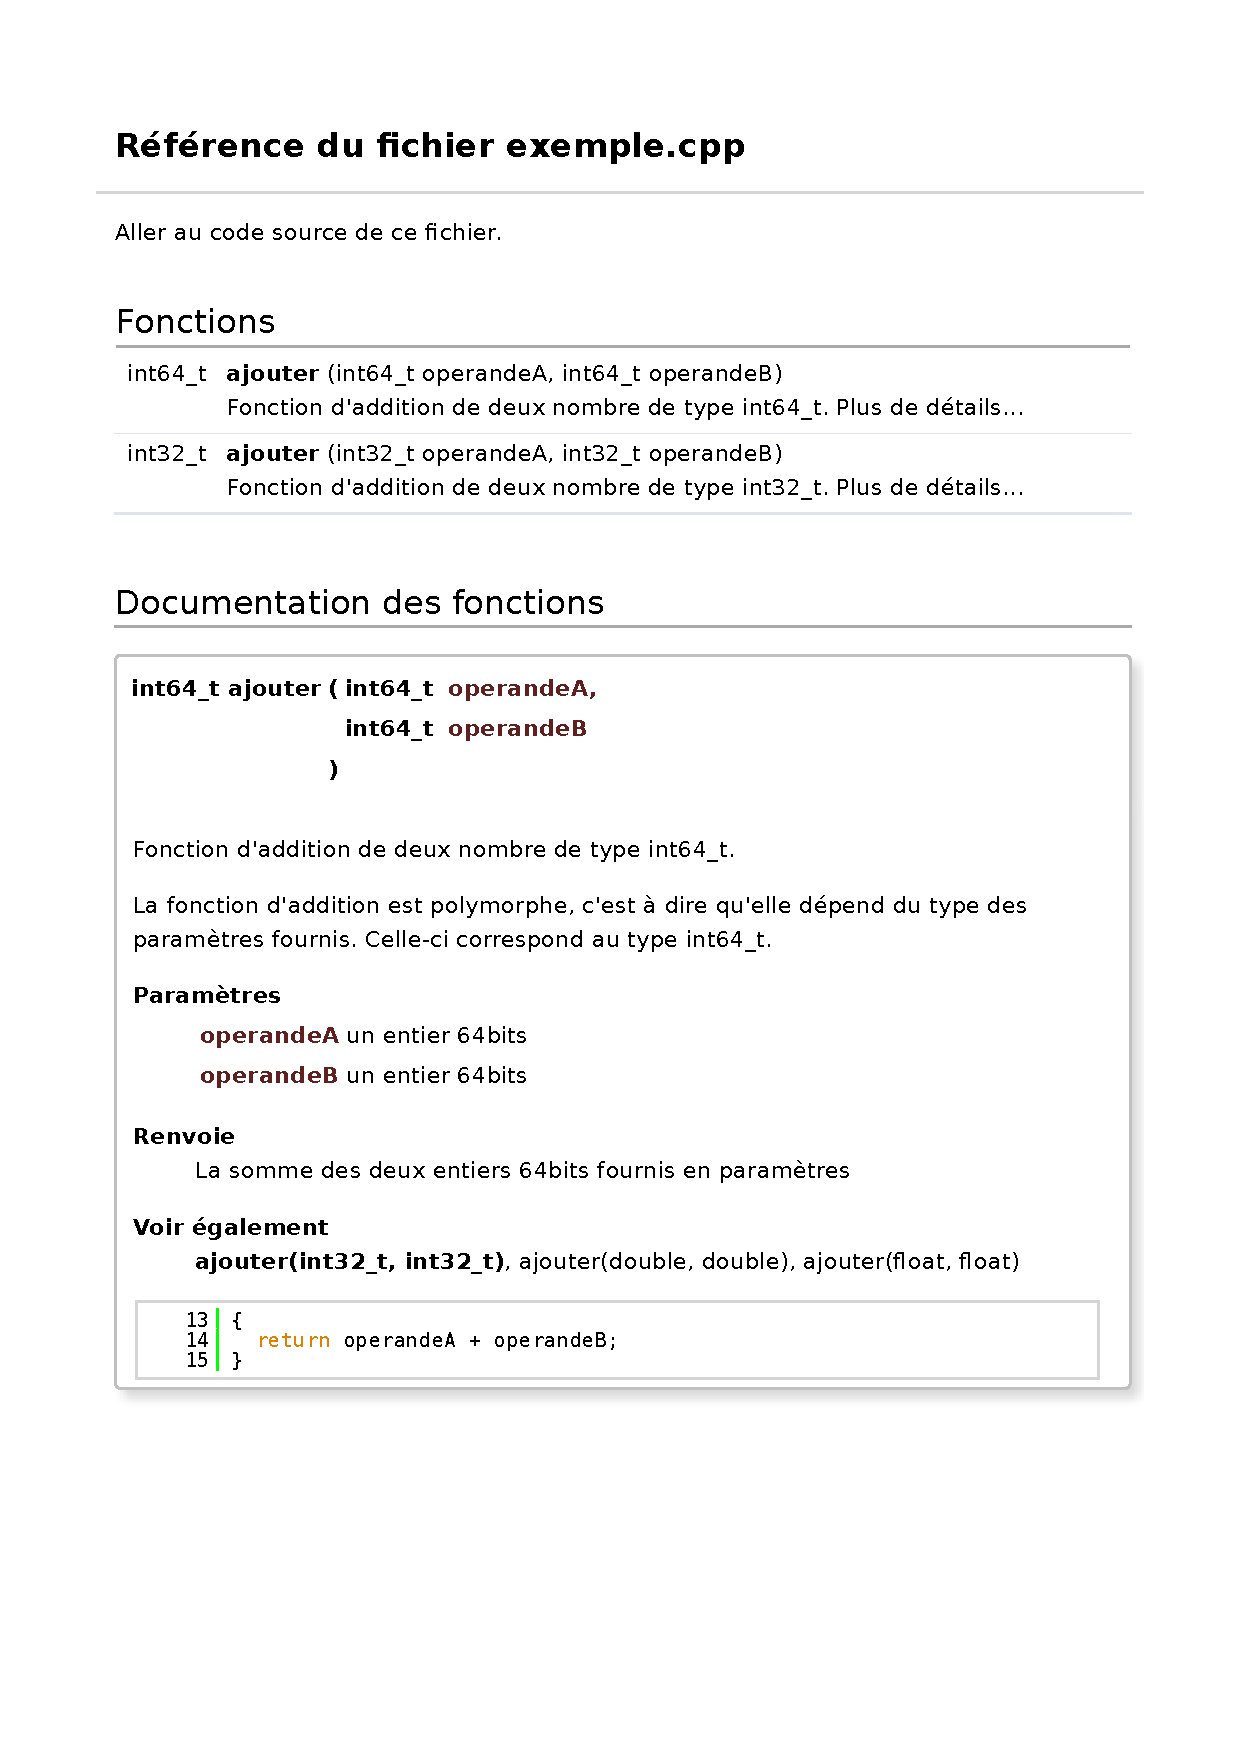
\includepdf[nup=1x2,landscape=true,pages=-]{export_html_doxygen.pdf}

\subsection{Documentation générée en \LaTeX}
\label{annexe:latexOutputDoc}
La configuration de \gls{doxygen} pour la sortie \LaTeX :
\lstset{caption={Extrait de la configuration \LaTeX de \gls{doxygen} du fichier \texttt{Doxyfile}},label={lst:doxyfileLATEX}}
\bash[stdout]
egrep "^([^#].*_L|L)ATEX.*" Doxyfile
\END

La documentation ainsi générée est un ensemble de fichiers \LaTeX et
un fichier de construction : \lstinline{Makefile}. La lecture de la
documentation ne peut se faire que si l'on compile les fichiers \LaTeX
en une sortie PDF par exemple.
\lstset{caption={Contenu du répertoire de la documentation \LaTeX}}
\bash[stdout]
ls doc/latex
\END

\begin{lstlisting}[style=groolotScript,caption={Instruction pour compiler la documentation \LaTeX en PDF}]
lambda@linux:~/repertoireProjet> cd doc/latex
lambda@linux:~/repertoireProjet> make
lambda@linux:~/repertoireProjet> evince refman.pdf
\end{lstlisting}

\includepdf[nup=1x2,landscape=true,pages={7-8}]{doc/latex/refman.pdf}

% References bibliographiques
\newpage \printbibheading
\printbibliography[nottype=online,check=notonline,heading=subbibliography,title={Bibliographiques}]
\printbibliography[check=online,heading=subbibliography,title={Webographiques}]

\printglossaries

\end{document}

